% CRITERIA	(2-3 pages)
	% -Check that each claim in the intro is addressed
	% -Forward reference evidence from a claim
	% -Present the experiments
	% -Analyze raw data
	
% OUTLINE
	% - Setup
		% - Criteria (Fitness)
			% - Distance (low weight since it doesn't really matter)
			% - Obstacle avoidance (Hight weight, mission critical)
			% - Minimize jerk (Mid weight)
		
		% - Touch breifly on encoding
			% - High order polynomial
			% - Chromozome - integer encoding
		% - Reporduction
			% - Random crossovers
		% - Mutation
			% - Defaults or Gusen's?
			% - Which worked out, why didn't the other?
		% - Initialization
			% - Random, pop size
		% - Termination
			% - Diversity convergence
			% - Or top half not coliding.
			% - Which worked out, why didn't the other?
			
		
	% - run with randomly generated environments (or at least 
		% - 1-5 objects
		% - placed randomly w/o overlap
		% - varying but constrained size
		% - fized start/end points
		% - Run 1000 times
		% - analyze data
		% - store data (map and the resultant path)

The Genetic Algorithm (GA) formed the basis for the experiemnts. Significant effort was expended setting up the GA in advance of testing, since without a well structured algorithm, the testing was sure to show poor results. The GA was implemented on Matlab, using the built-in GA libraries in order to avoid unnecessary development. While the base functionality was used, there remained many design considerations.

\subsection{Criteria}

\subsection{Configuration Space}
Commanding a robotic manipulator's position is complicated by the fact that it cannot be specified is X-Y-Z coordinates, but rather must be commanded using joint angles. Not only is this not intuitive for a human, but existing planning techniques function using more standard X-Y or X-Y-Z coordinate systems. As such, the robot's workspace was converted into a Configuration Space. Figure \ref{fig:ws2cs} shows both the workspace and the configuration space for a 2-DOF robot in an arbitrary workspace. The robotic manipulator's two degrees of freedom are denoted by the blue and red lines (each DOF respectively). The alloable robot configurations denoted in the Configuration Space by whitespace, while collisions are denoted by black.

\begin{figure}[h]
	\centering
	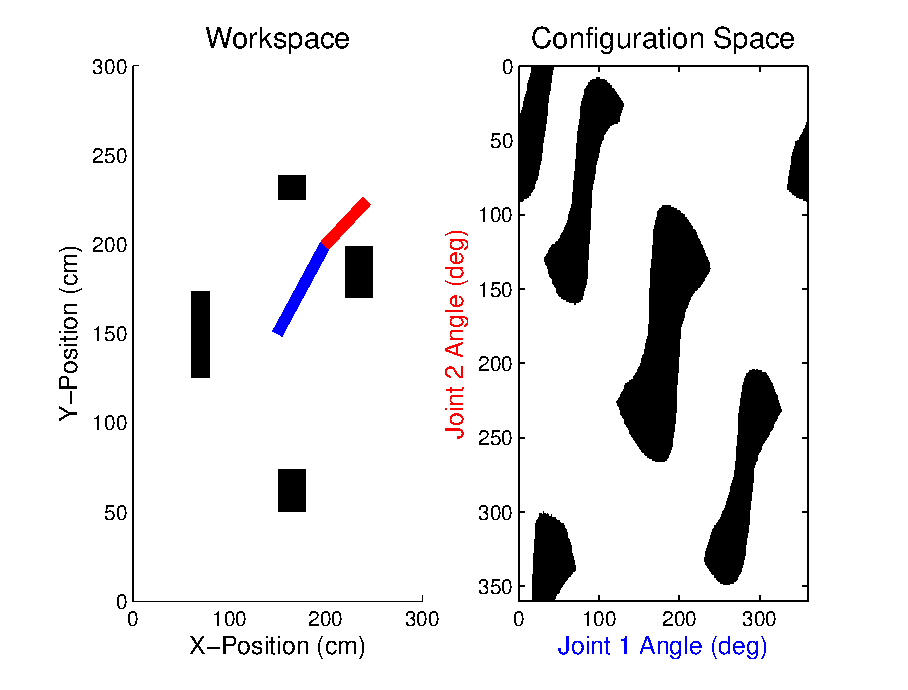
\includegraphics[width=3.5in]{./figures/wp2cs.eps}
	\caption{Conversion from robot workspace to configuration space }
	\label{fig:ws2cs}
\end{figure}

In the configuration space, robot tracjectories can be easily identified by either a human or a motion planning algorithm. This angle-angle plot can then be used to implement a polynomial trajectory, of which optimal coefficients can easily be solved using a Genetic Algorithm. The parameterized trajectory is denoted in Equation \ref{eq:polyTraj}.

\begin{align} \label{eq:polyTraj}
	\phi = P_4*\theta^4 + P_3*\theta^3 + P_2*\theta^2 + P_1*\theta + P_0
\end{align}

\subsection{Encoding}
The GA was developed using a linear encoding scheme, where a chromosome was defined to be an array of the polynomial function's coefficients (denoted as $\{P_0, \ldots, P_4\}$ in Equation \ref{eq:polyTraj}). Therefore, the GA would ultimately return the ideal set of coefficients for a function which would describe the optimal path for the robotic manipulator. These coefficients were limited to a range of [-50,50], since larger coefficients guarantee an invalid path since it would be too large and leave the workspace. While larger coefficients do not adversely affect the result of the algorithm, the increased diversity requires significantly larger computational resources which were not avaliable.

\subsection{Reproduction and Mutation}
/

\subsection{Initialization and Termination}



\textbf{SECTION REQUIREMENTS}
\begin{itemize}
\item Check that each claim in the intro is addressed
\item Forward reference evidence from a claim
\item Present the experiments
\item Analyze raw data
\end{itemize}